% !TEX TS-program = pdflatexmk
% mnras_template.tex
%
% LaTeX template for creating an MNRAS paper
%
% v3.0 released 14 May 2015
% (version numbers match those of mnras.cls)
%
% Copyright (C) Royal Astronomical Society 2015
% Authors:
% Keith T. Smith (Royal Astronomical Society)

% Change log
%
% v3.0 May 2015
%    Renamed to match the new package name
%    Version number matches mnras.cls
%    A few minor tweaks to wording
% v1.0 September 2013
%    Beta testing only - never publicly released
%    First version: a simple (ish) template for creating an MNRAS paper

%%%%%%%%%%%%%%%%%%%%%%%%%%%%%%%%%%%%%%%%%%%%%%%%%%

\documentclass[a4paper,fleqn,usenatbib]{mnras}

\usepackage{newtxtext,newtxmath}
\usepackage[T1]{fontenc}
\usepackage{ae,aecompl}
\usepackage{graphicx}	% Including figure files
\usepackage{amsmath}	% Advanced maths commands
\usepackage{amssymb}	% Extra maths symbols
\usepackage{bm}

\newcommand{\nb}{n_{\rm b}}
\newcommand{\prob}{{\rm P}}
\newcommand{\normal}{{\rm{N}}}
\newcommand{\uniform}{{\rm U}}
\newcommand{\dirichlet}{{\rm D}}
\newcommand{\invwish}{{\rm W}^{-1}}
\newcommand{\alphas}{{\bm a}}
\newcommand{\specmean}{{\bm m}}
\newcommand{\speccov}{{\bm S}}
\newcommand{\classprob}{{p}}
\newcommand{\classprobs}{{\bm p}}
\newcommand{\objspec}{{\bm s}}
\newcommand{\objclass}{{\kappa}}
\newcommand{\objclasses}{{\bm \kappa}}
\newcommand{\objdata}{\hat{\bm d}}
\newcommand{\objnoise}{{\bm N}}
\newcommand{\scalemat}{{\bm \Gamma}}
\newcommand{\wfmean}{{\bm w}}
\newcommand{\wfcov}{{\bm W}}

%%%%%%%%%%%%%%%%%%%%%%%%%%%%%%%%%%%%%%%%%%%%%%%%%%

\title[Gaussian Process Spectra]{Gaussian Process Spectra}
\author[S. M. Feeney et al.]{
Stephen M. Feeney,$^{1}$\thanks{E-mail: sfeeney@flatironinstitute.org}
Benjamin D. Wandelt,$^{1,2,3,4}$
and Melissa K. Ness$^{1,5}$
\\
$^{1}$Center for Computational Astrophysics, Flatiron Institute, 162 Fifth Avenue, New York, NY 10010, USA\\
$^{2}$Institut d'Astrophysique de Paris (IAP), UMR 7095, CNRS UPMC Universit\'e Paris 6, Sorbonne Universit\'es, \\
98bis boulevard Arago, F-75014 Paris, France\\
$^{3}$Institut Lagrange de Paris (ILP), UMR 7095, CNRS UPMC Universit\'e Paris 6, Sorbonne Universit\'es, \\
98bis boulevard Arago, F-75014 Paris, France\\
$^{4}$Department of Physics and Astronomy, University of Illinois at Urbana-Champaign, 1002 W Green St, Urbana, IL 61801, USA\\
$^{5}$Department of Astronomy, Columbia University, Pupin Physics Laboratories, New York, NY 10027, USA
}

% These dates will be filled out by the publisher
\date{Accepted XXX. Received YYY; in original form ZZZ}

% Enter the current year, for the copyright statements etc.
\pubyear{2019}

% Don't change these lines
\begin{document}
\label{firstpage}
\pagerange{\pageref{firstpage}--\pageref{lastpage}}
\maketitle

% Abstract of the paper
\begin{abstract}
This is a simple template for authors to write new MNRAS papers.
The abstract should briefly describe the aims, methods, and main results of the paper.
It should be a single paragraph not more than 250 words (200 words for Letters).
No references should appear in the abstract.
\end{abstract}

% Select between one and six entries from the list of approved keywords.
% Don't make up new ones.
\begin{keywords}
keyword1 -- keyword2 -- keyword3
\end{keywords}

%%%%%%%%%%%%%%%%%%%%%%%%%%%%%%%%%%%%%%%%%%%%%%%%%%

\section{Introduction}

Motivations/goals. By pooling information about stars we can:
\begin{enumerate}
\item Denoise to avoid excessively harsh signal-to-noise cuts. What is the current minimum S/N considered useful?
\item Inpaint masked regions of spectra to make, e.g., abundance measurements that would otherwise be impossible.
\item Determine the most informative regions of spectra to, e.g., determine whether we can retain sensitivity to abundances by observing a reduced spectral range.
\end{enumerate}

How will we do this? By modeling the spectra as a data-driven Gaussian Process. What is a GP and what are relevant applications.

%%%%%%%%%%%%%%%%%%%%%%%%%%%%%%%%%%%%%%%%%%%%%%%%%%

\section{Methods}

Describe Gaussian Process. True spectrum for each star is drawn from a GP with a mean spectrum and covariance matrix to be inferred from the data. We do not assume a kernel for our GP covariance, but rather infer the correlations between the observed spectral bins. This is so we can model the exact covariance and not worry about suboptimal choices of kernels caused by non-stationarity or different correlation lengths, line shapes, etc. The main downside of doing this is we can not make predictions for the spectra between the observed bins, though we could, given data observed on shifted or irregularly or different-spaced grids. We assume uninformative priors on the mean and covariance. We adopt an infinite uniform prior on the mean and a Jeffreys prior on the covariance matrix (precise form in notes).

Data are observed with Gaussian noise that is uncorrelated between spectral bins; masked pixels are assigned unit flux and effectively infinite noise uncertainties. These data, the inferred parameters, the likelihood and priors would fully specify the model if we had only one class. To account for the fact that the red clump might consist of multiple distinct populations (or one population whose distribution of true spectra is non-Gaussian) we allow for multiple classes to exist in our model. In this instance, each star is also assigned membership to a particular class. Class memberships are drawn from categorical distributions, with class probabilities drawn from a symmetric Dirichlet prior with concentration parameter $\alpha=1$.

The network diagram for our hierarchical Bayesian model is shown in Fig.~\ref{fig:network_diagram}, and the probability distributions defining each link are set out in Table.~\ref{tab:prob_dists}. The particular set of probability distributions chosen allow for the conditional distributions of each latent variable to be written analytically, and we hence use Gibbs sampling to estimate the joint posterior.

\begin{figure}
	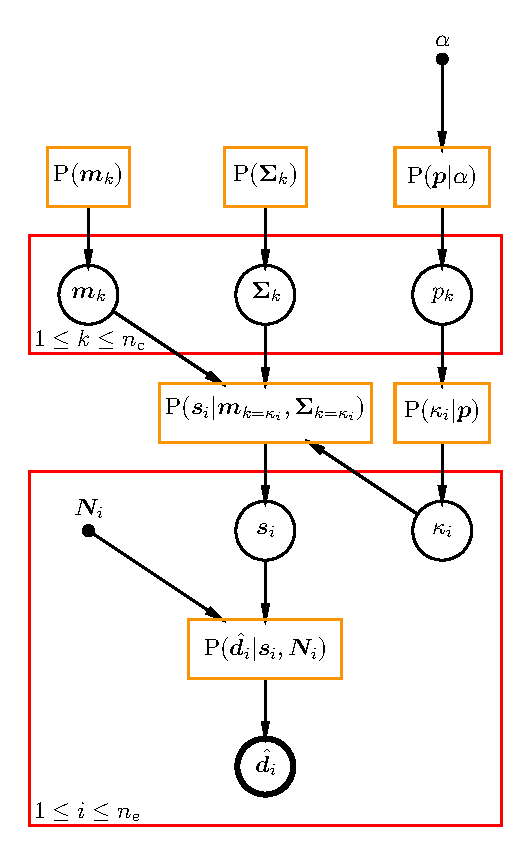
\includegraphics[width=\columnwidth]{bhm_plot.pdf}
    \caption{Network diagram for our hierarchical Bayesian model.}
    \label{fig:network_diagram}
\end{figure}

\begin{table*}
    \centering
    \caption{Priors, likelihoods and conditional distributions for Gibbs sampling. In our simplified notation, $\uniform$, $\dirichlet$, $\normal$ and $\invwish$ denote uniform, Dirichlet, normal and inverse-Wishart distributions, respectively.}
    \label{tab:prob_dists}
    \begin{tabular}{lll}
        \hline
        distribution & form & process \\
        \hline
        $\prob\left(\specmean_k\right)$ & $\uniform\left(-\infty,\infty\right)$ & Prior on $k^{\rm th}$ class's mean spectrum \\
        $\prob\left(\speccov_k\right)$ & $\left| \speccov \right|^{-\left(\nb+1\right)/2}$ & Prior on $k^{\rm th}$ class's spectrum covariance \\
        $\prob\left(\classprobs|\alpha\right)$ & $\dirichlet\left(\alpha\right)$ & Prior on class probabilities \\
        $\prob\left(\objspec_i|\specmean,\speccov,\objclass_i\right)$ & $\normal\left(\specmean_{k=\objclass_i},\speccov_{k=\objclass_i}\right)$ & $i^{\rm th}$ object's spectrum as Gaussian Process \\
        $\prob\left(\objclass_i = k|\classprobs\right)$ & $\classprob_k$ & $i^{\rm th}$ object's class membership \\
        $\prob\left(\objdata_i|\objspec_i,\objnoise_i\right)$ & $\normal\left(\objspec_i,\objnoise_i\right)$ & Noisy, masked spectral measurements \\
        \hline
        $\prob\left(\specmean_k | \speccov_k, \objspec, \objclasses \right)$ & $\normal \left( \frac{1}{n_k} \sum_{\objclass_i = k} \objspec_i, \frac{1}{n_k} \speccov_k \right)$ & Conditional on $k^{\rm th}$ class's mean spectrum \\
%        $\prob\left(\speccov_k | \specmean_k, \objspec, \objclasses \right)$ & $\left| \speccov_k \right|^{-(n_k + \nb + 1)/2} \exp \left( -\frac{1}{2} {\rm tr} \left[ \scalemat_k \speccov_k^{-1} \right] \right)$, where & Conditional on $k^{\rm th}$ class's spectrum covariance \\
        $\prob\left(\speccov_k | \specmean_k, \objspec, \objclasses \right)$ & $\invwish \left(n_k, \scalemat_k \right)$, where & Conditional on $k^{\rm th}$ class's spectrum covariance \\
         & $\scalemat_k = \sum_{\objclass_i = k} \left( \objspec_i - \specmean_k \right) \otimes \left( \objspec_i - \specmean_k \right)$ & \\
        $\prob\left(\classprob_k | \objclasses, \alpha\right)$ & $\dirichlet\left(\alphas\right)$, where $a_k = \alpha + n_k$ & Conditional on class probabilities \\
        $\prob \left( \objspec_i | \specmean_{k=\objclass_i}, \speccov_{k=\objclass_i}, \objdata_i, \objnoise_i \right)$ & $\normal \left( \wfmean_i, \wfcov_i \right)$, where & Conditional on $i^{\rm th}$ object's spectrum \\
         & $\wfcov_i = \left( \speccov_{k=\objclass_i}^{-1} + \objnoise_i^{-1} \right)^{-1}$ and &  \\
         & $\wfmean_i = \wfcov_i \left( \speccov_{k=\objclass_i}^{-1} \specmean_{k=\objclass_i} + \objnoise_i^{-1} \objdata_i \right)$ &  \\
        $\prob \left( \objclass_i = k | \specmean, \speccov, \classprobs \right)$ & $ \frac{ \exp \left( -\frac{1}{2} \left[ \chi^2_{i,k} + \ln \left| \speccov_k \right| \right] + \ln \classprob_k \right) }{ \sum_{k^\prime} \exp \left( -\frac{1}{2} \left[ \chi^2_{i,k^\prime} + \ln \left| \speccov_{k^\prime} \right| \right] + \ln \classprob_{k^\prime} \right) }$, where  & Conditional on $i^{\rm th}$ object's class membership \\
         & $\chi^2_{i,k} = \left( \objspec_i - \specmean_k \right)^T \speccov_k^{-1} \left( \objspec_i - \specmean_k \right) $ &  \\
        \hline
    \end{tabular}
\end{table*}

%%%%%%%%%%%%%%%%%%%%%%%%%%%%%%%%%%%%%%%%%%%%%%%%%%

\section{Data}

We take 29502 red clump stars identified in the APOGEE dataset. The contamination from non-red-clump stars is expected to be on the order of X percent.Describe pre-processing. The spectra cover the range 15100.80-16999.81 \AA, using $\nb = 8575$ spectral bins. Inversion of the resulting $\nb \times \nb$ covariance matrices would be too slow to permit inference, and we thus restrict our analysis to a set of spectral windows centred on lines confidently assigned to individual elements. Specifically, we process all spectral bins within $\pm2.5$ \AA\ of the line centres tabulated in Table~\ref{tab:window_centres}, reducing the number of spectral bins to $\nb = 557$ and hence inversion time by a factor of $\sim3500$.

\begin{table}
    \centering
    \caption{Elemental windows.}
    \label{tab:window_centres}
    \begin{tabular}{lcc}
        \hline
        element & window & window \\
         & centre 1 & centre 2 \\
        \hline
        Al & 15972.905 & - \\
        C & 15479.107 & 15582.101 \\
        Ca & 16161.807 & - \\
        Cu & 16010.023 & - \\
        Fe & 15494.733 & 15505.643 \\
        Mg & 15425.309 & 15697.701 \\
        Mn & 15162.885 & 15221.867 \\
        N & 15161.42 & 15321.871 \\
        Na & 16393.443 & - \\
        Ni & 15559.517 & 15758.315 \\
        O & 15269.893 & 15631.468 \\
        Si & 15365.335 & 15964.753 \\
        Ti & 15190.779 & 15339.241 \\
        Ce & 15789.063 & 16380.954 \\
        Nd & 16058.014 & - \\
        \hline
    \end{tabular}
\end{table}

%%%%%%%%%%%%%%%%%%%%%%%%%%%%%%%%%%%%%%%%%%%%%%%%%%

\section{Results}

Even more stuff.

\begin{figure}
	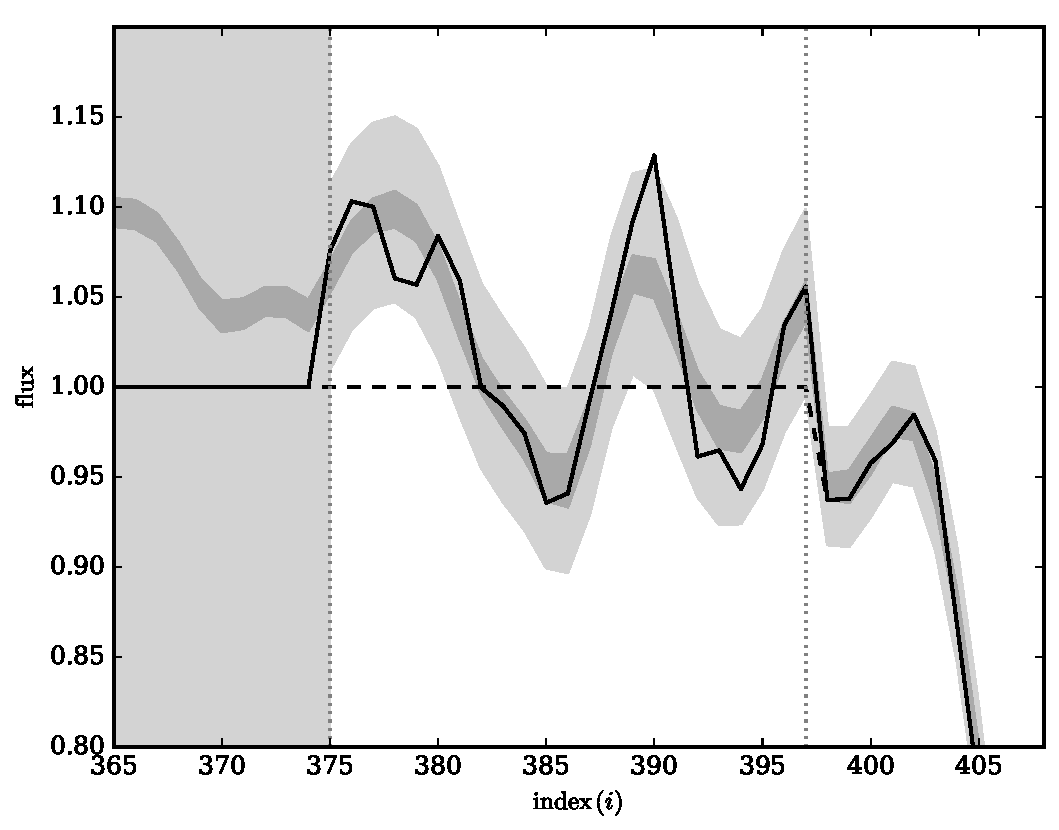
\includegraphics[width=\columnwidth]{apogee_centers_subset2_ce_nd_29502_spc_rec_test_recovery_zoom.pdf}
    \caption{Recovery test. Artificially masking the 15789 \AA\ Cerium window (indicated by vertical dotted lines) for the lowest-SNR star results in an inferred true spectrum (dark-grey shaded region) that is entirely in agreement with the measurement (solid black line) once noise is taken into account (light-grey shaded region).}
    \label{fig:recovery_test}
\end{figure}

\begin{figure*}
	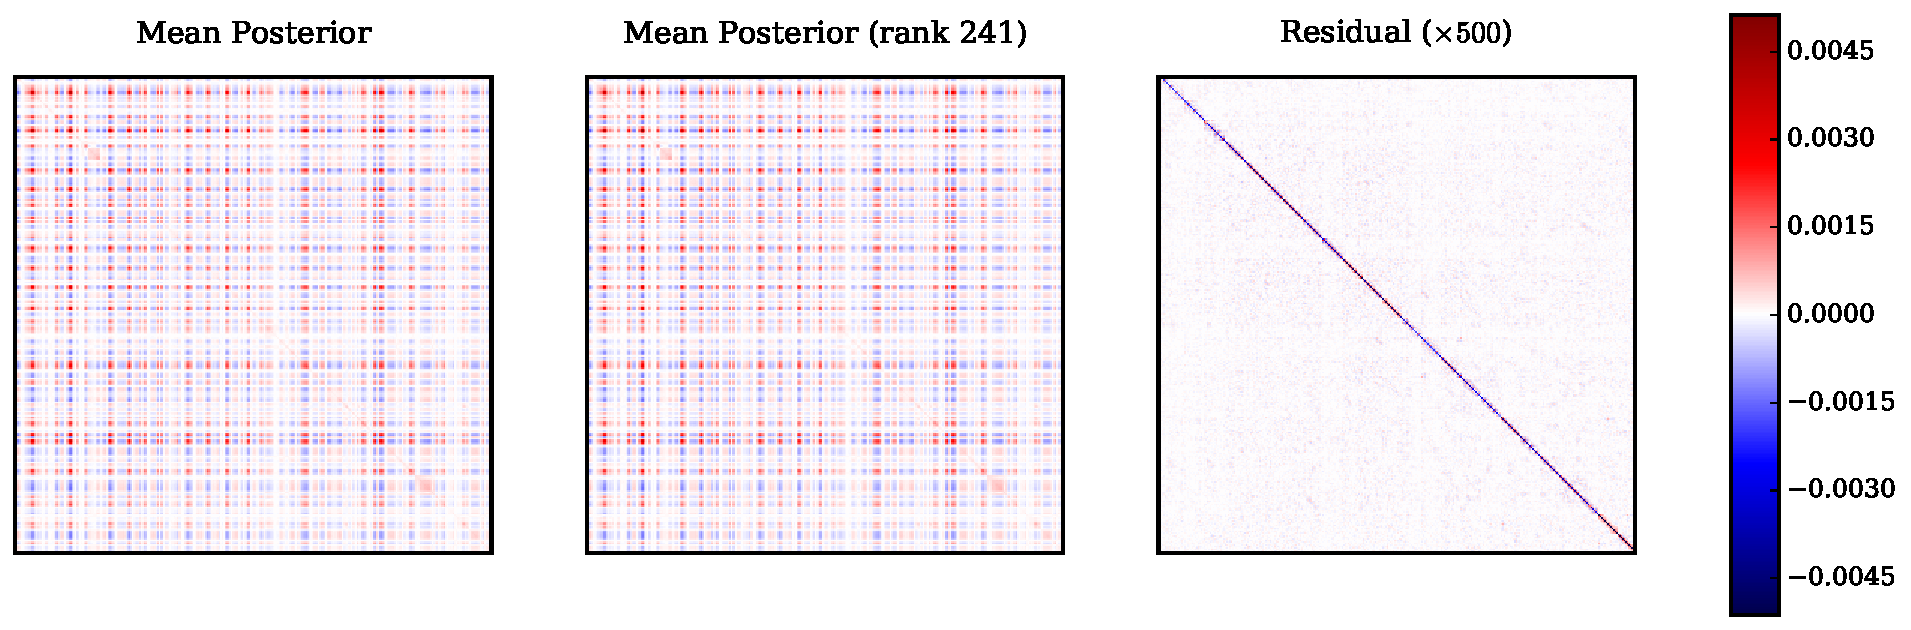
\includegraphics[width=2\columnwidth]{apogee_centers_subset2_ce_nd_29502_spc_low_rank_covariance.pdf}
    \caption{Mean-posterior covariance matrix (left), its low-rank approximation (centre) constructed from all eigenvectors with eigenvalues within $10^{-4}$ of the largest, and the residuals (right).}
    \label{fig:inferred_cov}
\end{figure*}

\begin{figure*}
	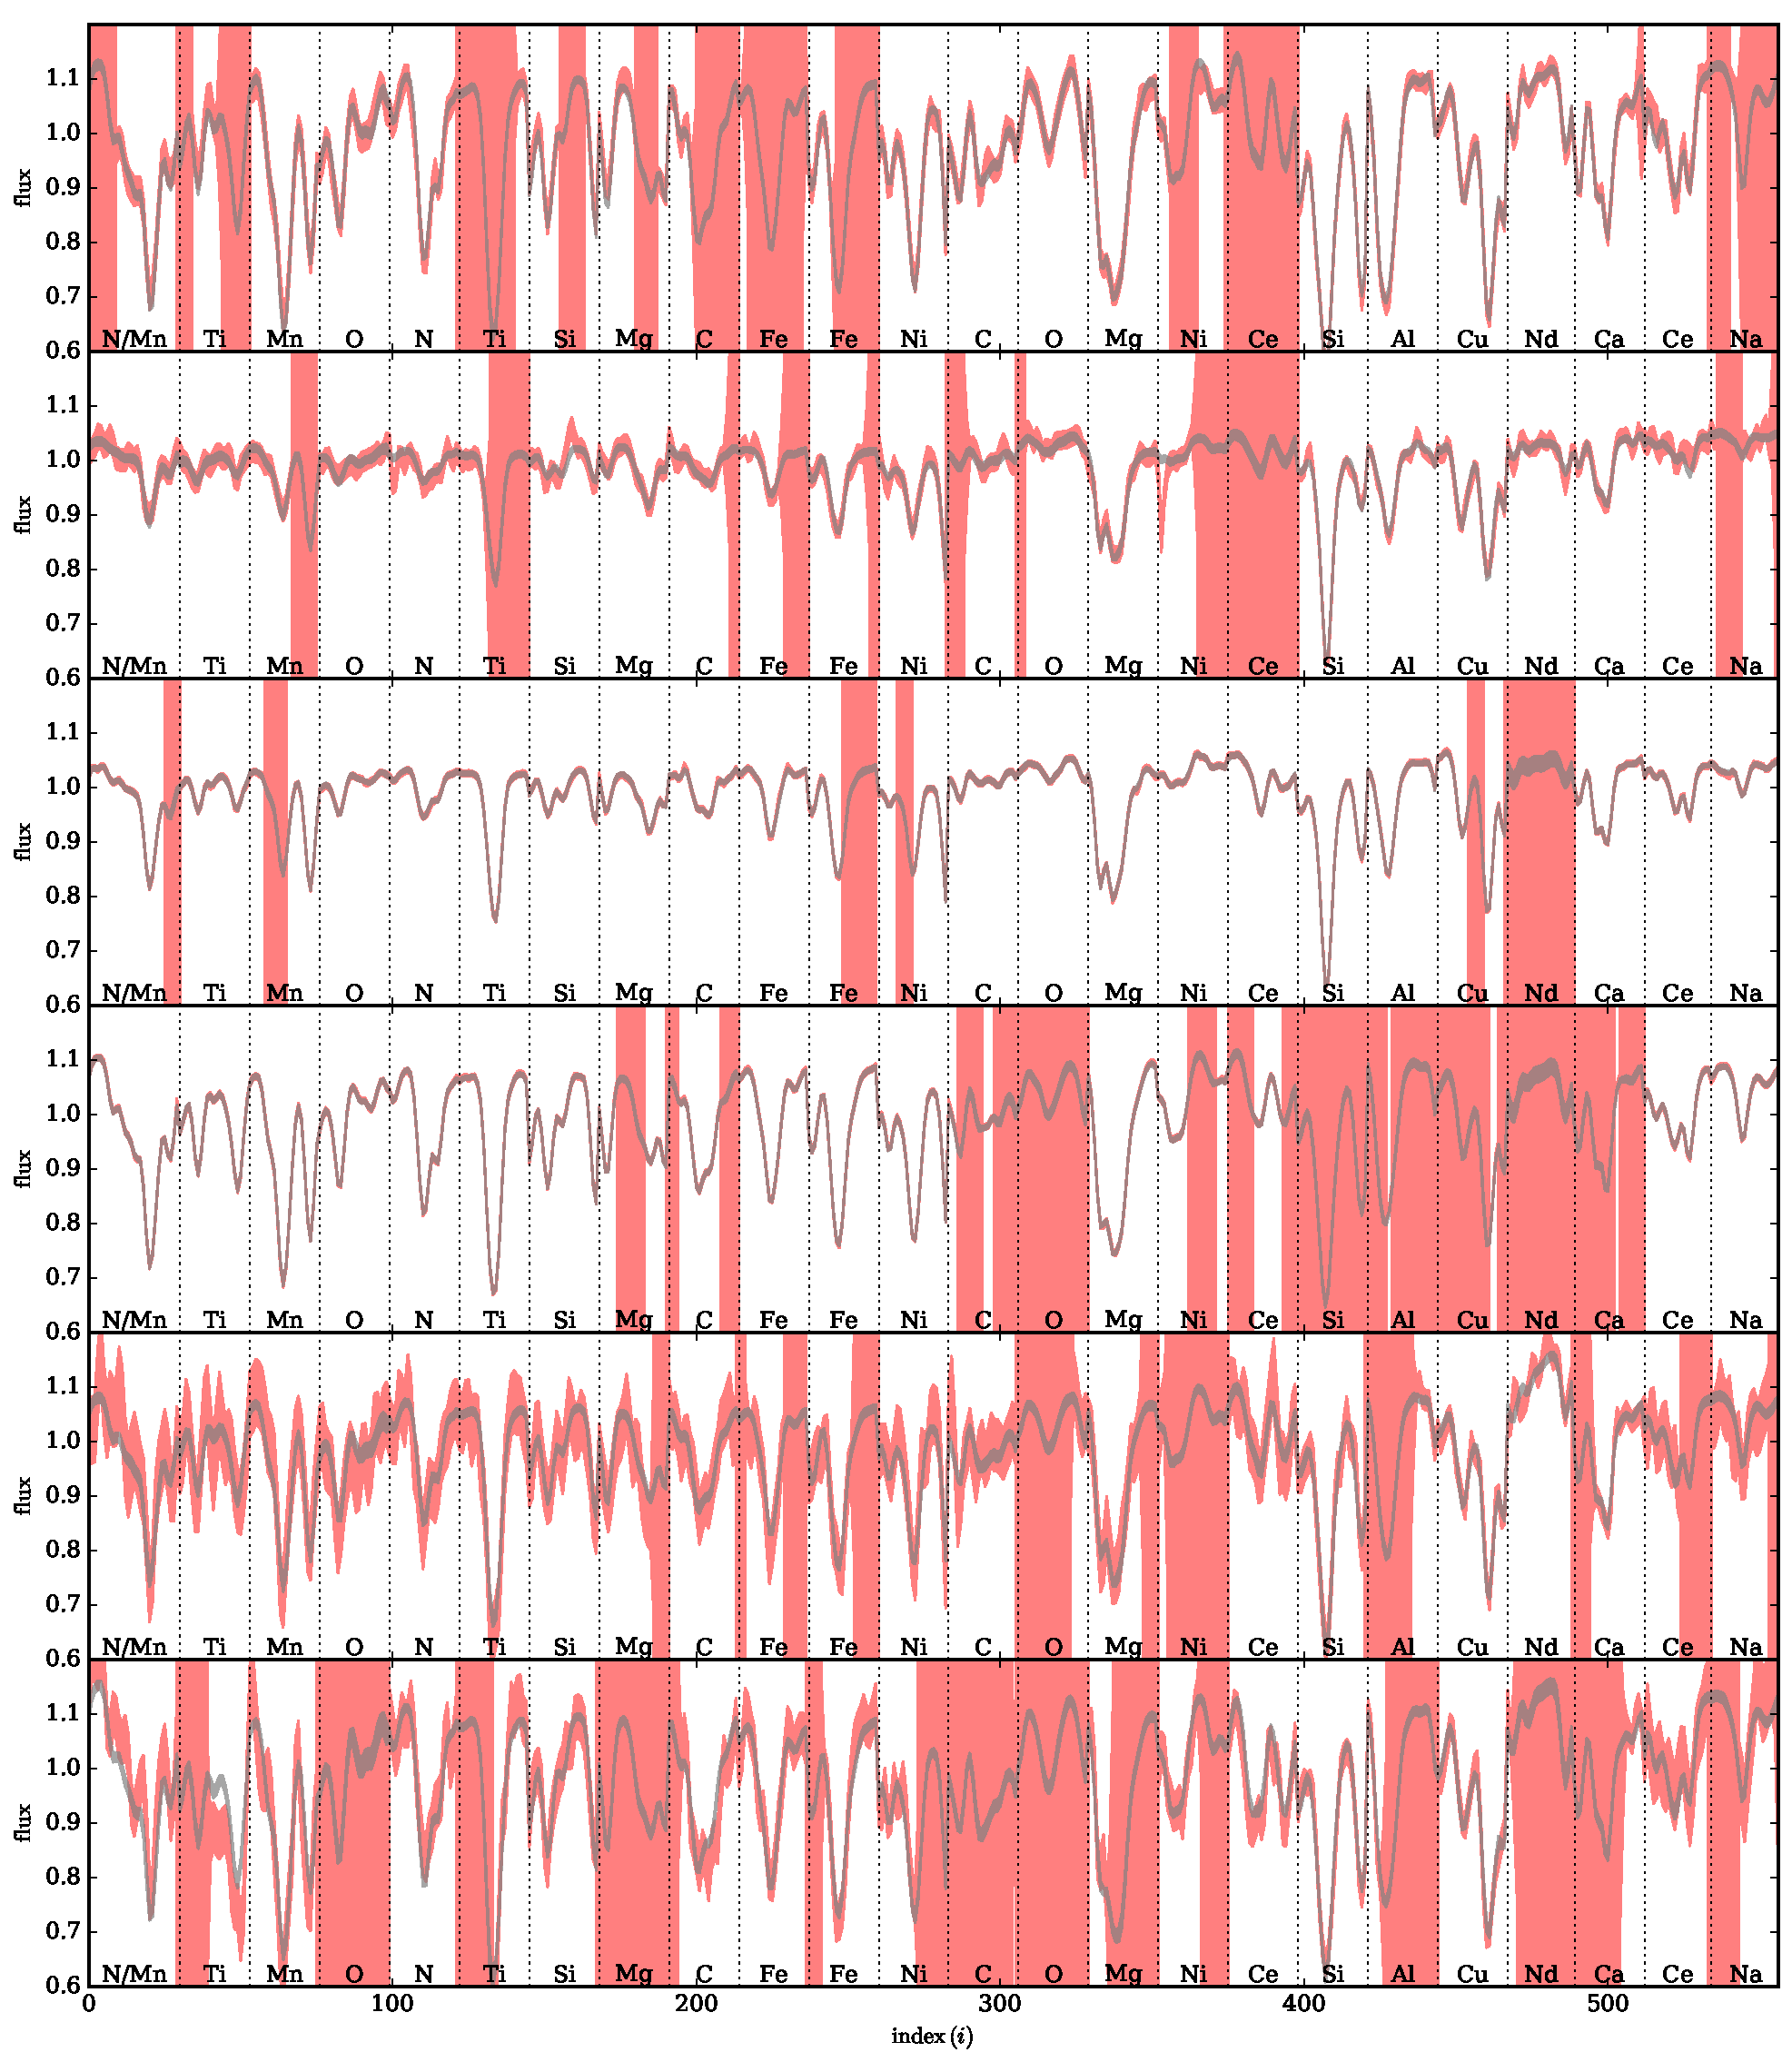
\includegraphics[width=2\columnwidth]{apogee_centers_subset2_ce_nd_29502_spc_save_spectra.pdf}
    \caption{Observed spectra (pink shaded regions) and inferred ``true'' spectra (grey shaded regions) for six interesting examples illustrating our ability to inpaint and denoise. From top: two spectra with the 15789 \AA\ Cerium window fully masked; two spectra with the 16058 \AA\ Neodymium window fully masked; the two lowest signal-to-noise spectra.}
    \label{fig:inpainting_denoising_examples}
\end{figure*}

\begin{figure*}
	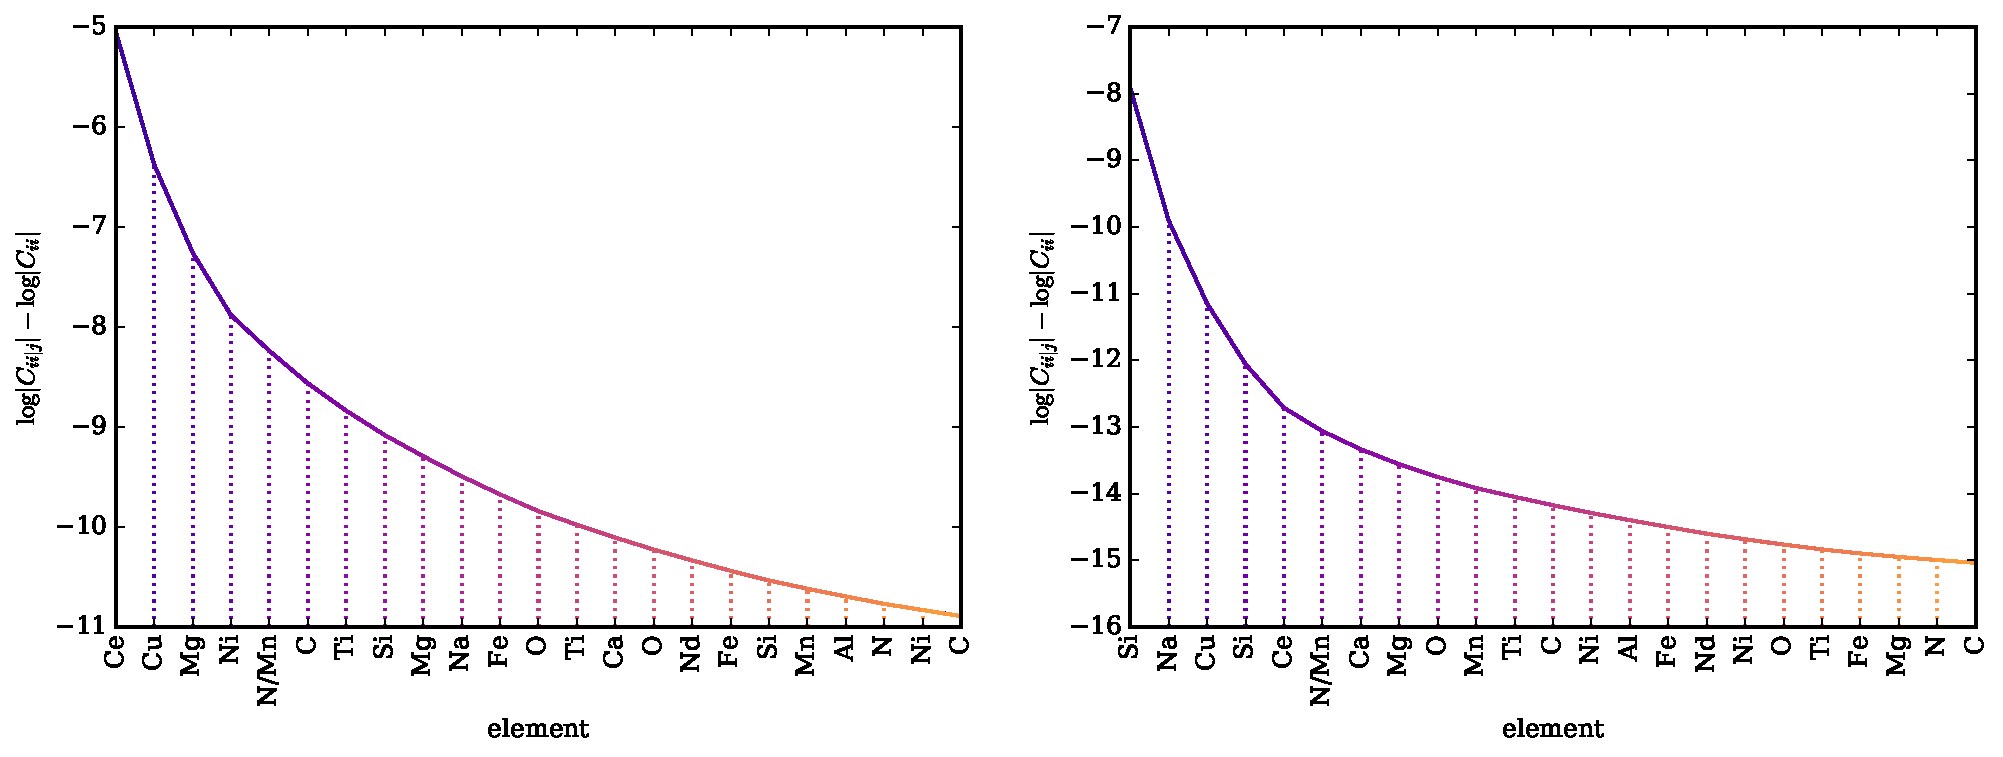
\includegraphics[width=2\columnwidth]{apogee_centers_subset2_ce_nd_29502_spc_ce_inf_gain.pdf}
	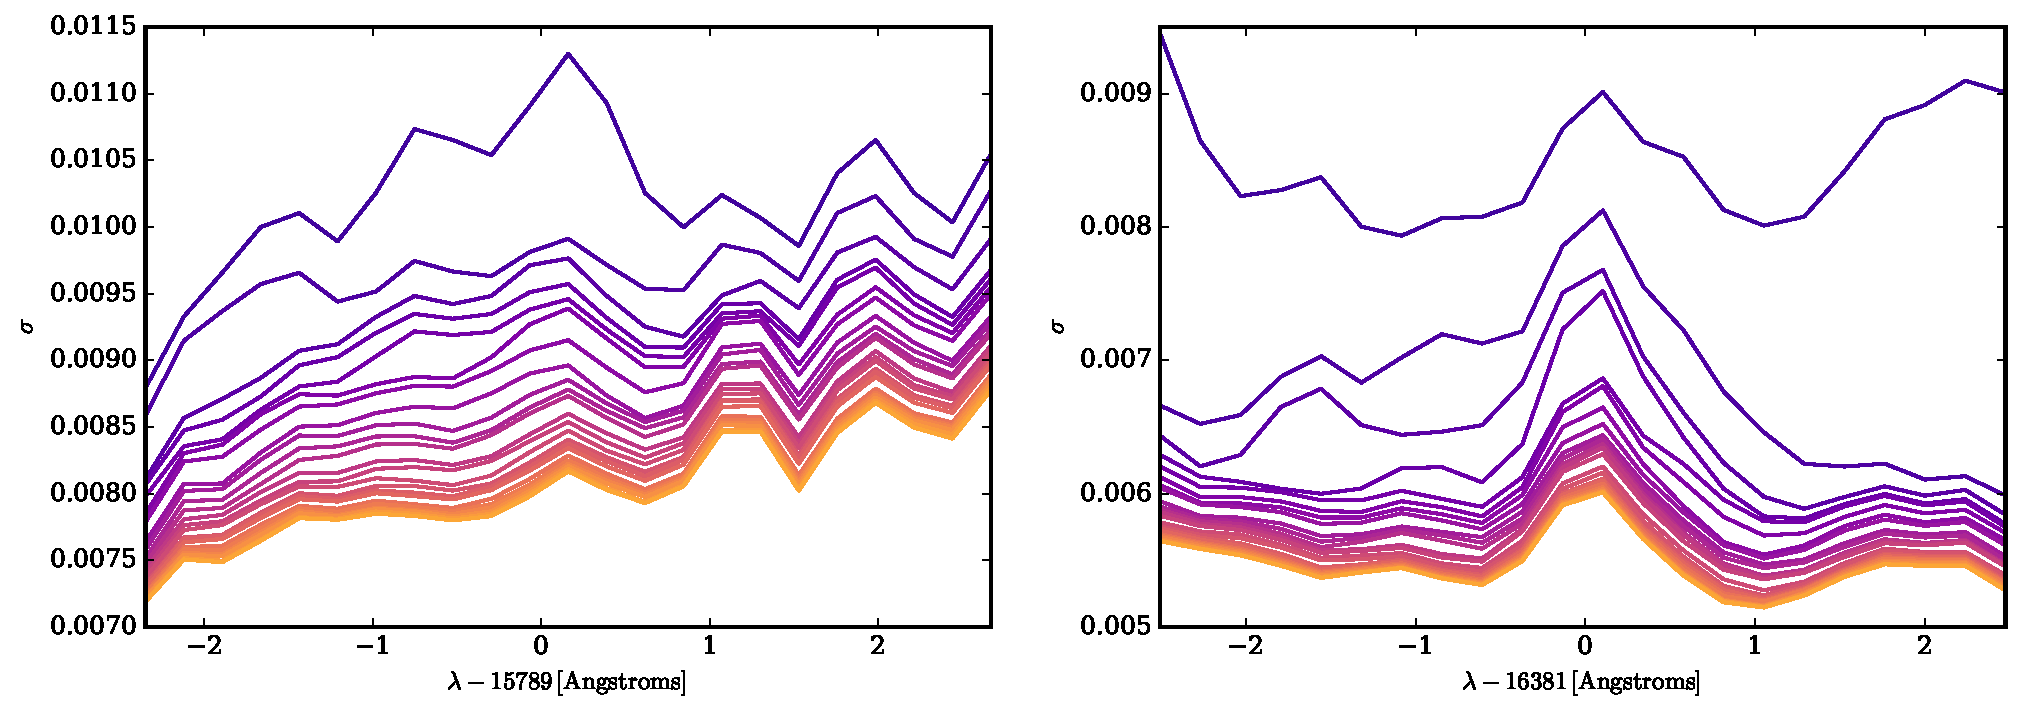
\includegraphics[width=2\columnwidth]{apogee_centers_subset2_ce_nd_29502_spc_ce_conditional_stddevs.pdf}
    \caption{Information gain (top) and conditional standard deviation (bottom) for Cerium windows given observations of other elemental windows. The uncertainty on the predicted spectrum without observations of other windows is shown in black.}
    \label{fig:ce_information}
\end{figure*}

\begin{figure}
	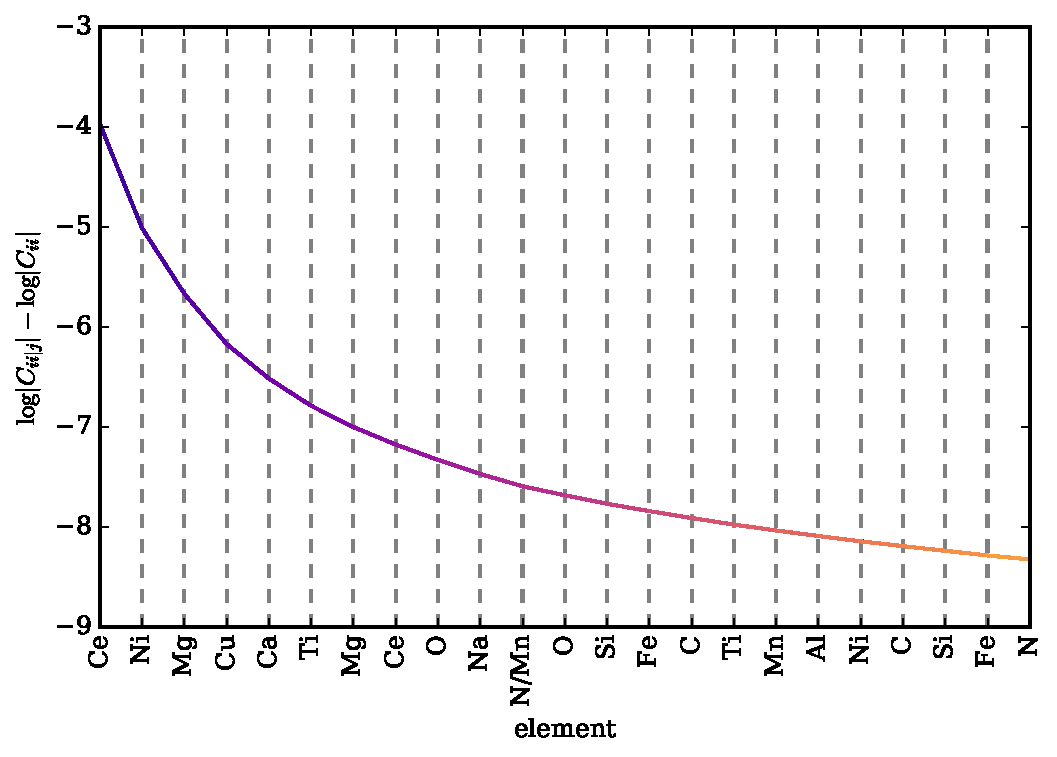
\includegraphics[width=\columnwidth]{apogee_centers_subset2_ce_nd_29502_spc_nd_inf_gain.pdf}
	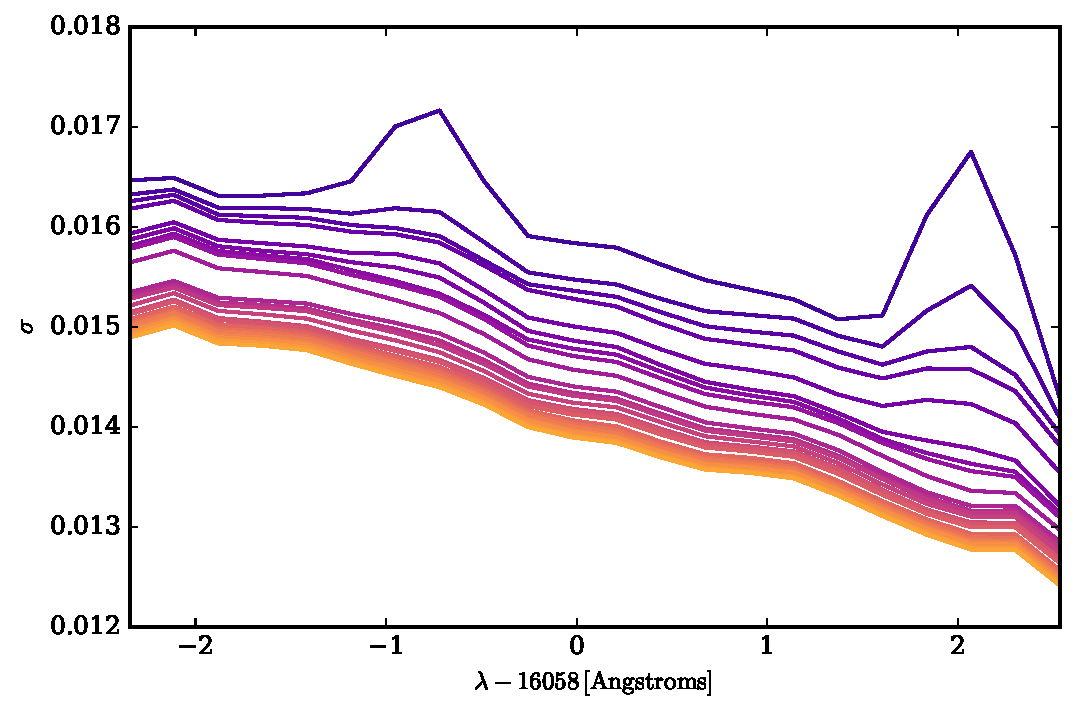
\includegraphics[width=\columnwidth]{apogee_centers_subset2_ce_nd_29502_spc_nd_conditional_stddevs.pdf}
    \caption{Information gain (top) and conditional standard deviation (bottom) for Neodymium window given observations of other elemental windows. The uncertainty on the predicted spectrum without observations of other windows is shown in black.}
    \label{fig:nd_information}
\end{figure}

%%%%%%%%%%%%%%%%%%%%%%%%%%%%%%%%%%%%%%%%%%%%%%%%%%

\section{Conclusions}

TBD.

%%%%%%%%%%%%%%%%%%%%%%%%%%%%%%%%%%%%%%%%%%%%%%%%%%

\section*{Acknowledgements}

The Flatiron Institute is supported by the Simons Foundation.

%%%%%%%%%%%%%%%%%%%%%%%%%%%%%%%%%%%%%%%%%%%%%%%%%%

%\bibliographystyle{mnras}
%\bibliography{example} % if your bibtex file is called example.bib

%%%%%%%%%%%%%%%%%%%%%%%%%%%%%%%%%%%%%%%%%%%%%%%%%%


% Don't change these lines
\bsp	% typesetting comment
\label{lastpage}
\end{document}

% End of mnras_template.tex